\paragraph{La classe DealerManager}


\begin{minipage}
    {\linewidth}
    \centering
    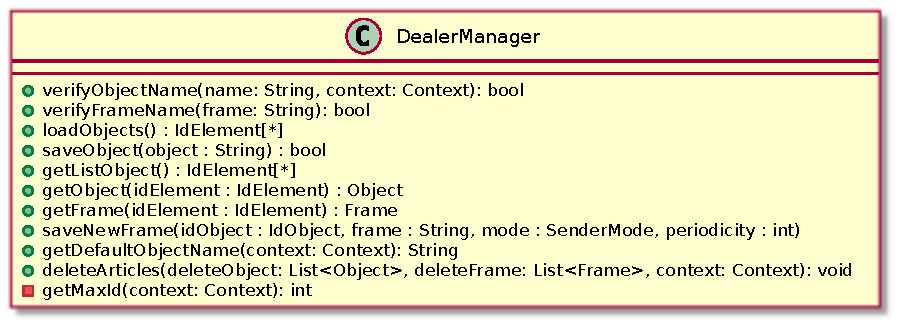
\includegraphics[width=0.80\linewidth]{../schemas/Conception_detaillee/classe_dealer.pdf}
    \captionof{figure}{Diagramme de classe de DealerManager}
\end{minipage}
\subparagraph{Philosophie de conception \newline} 

\medspace

La classe DealerManager permet d'enregistrer les objets et trames enregistrés sur l'application CANdroid. Les opérations étant déjà détaillées dans la conception générale, nous nous contenterons de les lister.
\subparagraph{Description structurelle \newline}

\medspace

\textbf{Attributs :}

N.A.

\textbf{Services offerts :}

\begin{itemize}
    \item \textbf{verifyObjectName(name: String, context: Context): bool}  
    \item \textbf{verifyFrameName(frame: String): bool}
    \item \textbf{loadObjects() : IdElement[*]}  
    \item \textbf{saveObject(object : String) : bool}  
    \item \textbf{getListObject() : IdElement[*]}  
    \item \textbf{getObject(idElement : IdElement) : Object}  
    \item \textbf{getFrame(idElement : IdElement) : Frame}  
    \item \textbf{saveNewFrame(idObject : IdObject, frame : String, mode : SenderMode, periodicity : int)}  
    \item \textbf{getDefaultObjectName(context: Context): String}
    \item \textbf{deleteArticles(deleteObject: List<Object>, deleteFrame: List<Frame>, context: Context): void} 
    \item \textbf{getMaxId(context: Context): int}
\end{itemize}

